% --------------------------------------------------------------
% This is all preamble stuff that you don't have to worry about.
% Head down to where it says "Start here"
% --------------------------------------------------------------
 
\documentclass[12pt]{article}
 
\usepackage[nouppercase,headsepline,footsepline,plainfootsepline]{scrpage2}
\automark{section}
\pagestyle{scrheadings}
%\clearscrheadfoot
\ihead{Compact Sets}
%\ofoot[\pagemark]{\pagemark}% Optional argument controls chapter-starting pages
\ifoot[(Author)]{{\sl \hfill Meenmo K.}}

\usepackage[margin=1in]{geometry} 
\usepackage{amsmath,amsthm,amssymb,scrextend}
\usepackage{fancyhdr}
\usepackage{enumitem}
\usepackage{amsmath}
\usepackage{amssymb}
\usepackage{textcomp}
\usepackage{fancybox}
\usepackage{tikz}
\usepackage{cancel}
\usepackage{tasks}


\newcommand{\N}{\mathbb{N}}
\newcommand{\Z}{\mathbb{Z}}
\newcommand{\I}{\mathbb{I}}
\newcommand{\R}{\mathbb{R}}
\newcommand{\Q}{\mathbb{Q}}
\renewcommand{\qed}{\hfill$\blacksquare$}
\let\newproof\proof
\renewenvironment{proof}{\begin{addmargin}[1em]{0em}\begin{newproof}}{\end{newproof}\end{addmargin}\qed}
% \newcommand{\expl}[1]{\text{\hfill[#1]}$}
\setlength{\parindent}{0pt}
\newenvironment{theorem}[2][Theorem]{\begin{trivlist}
\item[\hskip \labelsep {\bfseries #1}\hskip \labelsep {\bfseries #2.}]}{\end{trivlist}}
\newenvironment{lemma}[2][Lemma]{\begin{trivlist}
\item[\hskip \labelsep {\bfseries #1}\hskip \labelsep {\bfseries #2.}]}{\end{trivlist}}
\newenvironment{problem}[2][Problem]{\begin{trivlist}
\item[\hskip \labelsep {\bfseries #1}\hskip \labelsep {\bfseries #2.}]}{\end{trivlist}}
\newenvironment{exercise}[2][Exercise]{\begin{trivlist}
\item[\hskip \labelsep {\bfseries #1}\hskip \labelsep {\bfseries #2.}]}{\end{trivlist}}
\newenvironment{reflection}[2][Reflection]{\begin{trivlist}
\item[\hskip \labelsep {\bfseries #1}\hskip \labelsep {\bfseries #2.}]}{\end{trivlist}}
\newenvironment{proposition}[2][Proposition]{\begin{trivlist}
\item[\hskip \labelsep {\bfseries #1}\hskip \labelsep {\bfseries #2.}]}{\end{trivlist}}
\newenvironment{corollary}[2][Corollary]{\begin{trivlist}
\item[\hskip \labelsep {\bfseries #1}\hskip \labelsep {\bfseries #2.}]}{\end{trivlist}}
 
 
\begin{document}
\section{Compact Sets}

\begin{block}{\bf Def}
Let $(X,d)$ be a metric space, $K\subset X$. An {\bf open cover} of $K$ is a collection $\{G_\alpha\}$ of open sets such that $K\subset \bigbigcup\limits_\alpha G_\alpha$
\end{block}


\vspace{1.5\baselineskip}
\begin{block}{\bf Def}
Let $K\subset X$. $K$ is {\bf compact} if every open cover$\{G_\alpha\}$ of $K$ has a finite subcover.\\
i.e. $\exists\; \alpha_1,...,\alpha_n$ such that $K\subset \bigcup\limits_{\alpha=1}^n G_\alpha$
\end{block}

\begin{itemize}
    \item In order to show a given set is compact, there exists a set of {\sl finite open covers} has to have finite sub-covers.
    
    \item If it is not compact, there is a single open cover that has no finite sub-cover.
\end{itemize}

\begin{block}{\bf Example}: Compact
\begin{itemize}
    \item Let $K=[0,1], X = \mathbb{R}$
    \item Consider $\{G_\alpha\}\cup\{G_0\}\cup\{G_1\}$ where
        \begin{enumerate}[label=(\roman*)]
            \item $G_\alpha = (\frac{\alpha}{2},1)\;\forall\;\alpha\in(0,1)$
            \item $G_0 = (-\epsilon, \epsilon)$
            \item $G_1 = (1-\epsilon, 1+\epsilon)$ for some $\epsilon > 0$
        \end{enumerate}
    \item Then $\{G_\alpha\}\cup\{G_0\}\cup\{G_1\}$ is an open cover of [0,1].
    \item It has finite subcovers $\{G_\alpha,G_0,G_\epsilon\}$
    \item Thus $K = [0.1]$ is compact.
\end{itemize}
\end{block}

\vspace{1.5\baselineskip}
\begin{block}{\bf Example}: Not Compact\\
Let $E = (0,1),\; X=\mathbb{R}$
\begin{itemize}
    \item E is an open cover itself, but that does not mean it is compact.
    \item Let $G_\alpha = (\frac{\alpha}{2},1)\;\forall\;\alpha\in(0,1)$. Then $\{G_\alpha\}$ is open covers of $E$.
    \item But we are unable to take a finite collection of $G_\alpha$.
    \item Hence $E$ is not a compact set.
\end{itemize}
\end{block}


\newpage
\begin{block}{\bf Theorem} 
Suppose $K\subset Y\subset X$. Then $K$ is compact relative to $X$ if and only if $K$ is compact relative to $Y$.

\vspace{1.0\baselineskip}
{\sl Remark}: We know that any metric $(X,d)$ is both open and closed relative to itself. However, this is not true for compactness.
\end{block}

\vspace{1.0\baselineskip}
\begin{block}{\sl Proof} 
\begin{itemize}
    \item $\Rightarrow$ Suppose K is compact relative to Y.
    \item Let $\{G_\alpha\}$ be a collection of sets open relative to X. \;\;i.e. $K\subset \bigcup\limits_\alpha G_\alpha$
    \item Let $V_\alpha = G_\alpha \cap Y\;\; \forall\;\alpha$, so $V_\alpha$ is open relative to Y.
    \item For $K\subset Y$, $K=K \cap Y \subset \bigcup\limits_\alpha G_\alpha \cap Y = \bigcup\limits_\alpha V_\alpha$.
    \item So $V_\alpha$ is an open cover of K relative to Y.
    \item Hence, $\exists\; \alpha_1,...,\alpha_n$ such that $K\subset \cap\limits_{i=1}^n V_{\alpha_i}$
    \item Now $K\subset \bigcup\limits_{i=1}^n V_{\alpha_i} = 
    \bigcup\limits_{i=1}^n (G_{\alpha_i} \cap Y) \subset 
    \bigcup\limits_{i=1}^n G_{\alpha_i}$
    \item So K is compact relative to X.\\
    
    \item $\Leftarrow$ Suppose K is compact relative to X.
    \item Assume $V_\alpha$ is an open cover of K relative to Y and $G_\alpha$ is open in X \;\; i.e. $V_\alpha = G_\alpha \cap Y$.
    \item So $K\subset \bigcup\limits_\alpha V_\alpha \subset \bigcup\limits_\alpha G_\alpha$\;\; i.e. $G_\alpha$ is an open cover of K in X.
    \item As K is compact relative to X, $\exists\;\alpha_1,...,\alpha_n$ such that $K\subset \bigcup\limits_{i=1}^n G_{\alpha_i}$. \item Hence $K = K\cap Y \subset \bigcup\limits_{i=1}^n G_{\alpha_i} \cap Y = \bigcup\limits_{i=1}^n V_{\alpha_i}$ 
    \item Since $\exists\; V_{1},...,V_{\alpha}$ is a finite subcover, K is compact relative to Y.
\end{itemize}
\end{block}

\newpage
\begin{block}{\bf Theorem } Compact subsets $K$ of metric spaces $X$, $K\subset X$, are closed.\\
{\sl Note. Closed does not have to imply compactness, but compactness implies closed.\\
e.g. $\mathbb{R}$ is closed, but not compact.}\\

{\sl Proof.}
\begin{itemize}
    \item We shall prove that the complement of $K$, $K^c$, is an open subset of $X$.
    \item Suppose $p \in X,\; p\notin K,\text{ but } q \in K$.
    \item Let $V_q$ is neighborhoods of $p$ and $W_q$ is those of q whose radius is less than $\frac{d(p,q)}{2}$.
    \item Since $K$ is compact, there are {\bf finitely many} points $q_1,...,q_n$ in $K$ such that
    $$K \subset W_{q_1} \cup \ldots \cup W_{q_n} = W$$
    \item If $V= V_{q_1} \cap \ldots \cap V_{q_1}$, then $V$ is a neighborhood of $p$ which does not intersect $W$.
    \item Hence $V\subset K^c$, so that $p$ is an interior point of $K^c$.
   $$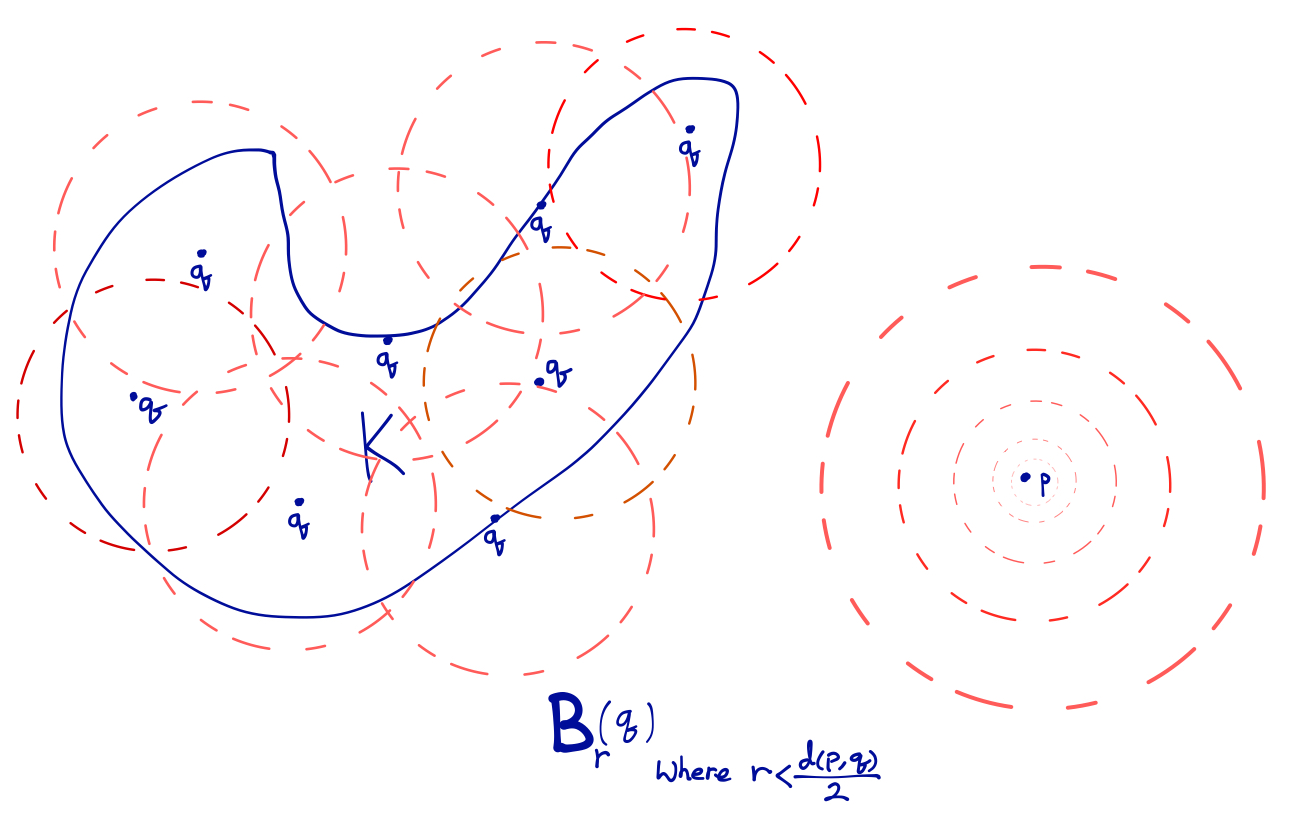
\includegraphics[height=6cm, width=10cm]{compact_1.jpg}$$
\end{itemize}
\end{block}

\vspace{1\baselineskip}
\begin{block}{\bf Theorem} Closed subsets of compact sets are compact.

\vspace{1\baselineskip}\\
{\sl Proof.}
\begin{itemize}
    \item Suppose $F\subset K\subset X$, $F$ is closed relative to $X$, and $K$ is compact.
    \item Let $\{V_\alpha\}$ be an open cover of F. 
    \item If $F^c$ is adjoined to $\{V_\alpha\}$, we obtain an open cover $\Omega$ of $K$.
    \item Since $K$ is compact, $\exists$ a finite subcollection $\Phi$ of $\Omega$ which overs $K$, and F also.
    \item If $F^c$ is a member of $\Phi$, we may remove it from $\Phi$ and still retain an open cover of $F$.
    \item We have thus shown that a finite subcollection of $\{V_\alpha\}$ covers $F$.\\
\end{itemize}
\end{block}

\begin{block}{\bf Corollary} If F is closed, K is compact, then $F\cap K$ is compact.\end{block}

\newpage
\begin{block}{\bf Theorem} If $\{K_\alpha\}$ is a collection of compact subsets of a metric space $X$ such that the intersection of every finite subcollection of $\{K_\alpha\}$ is nonempty, then $\bigcap K_\alpha$ is nonempty.\\ \end{block}

\begin{block}{\sl Proof.}
\begin{enumerate}[label=(\roman*)]
    \item Suppose by contradiction that $\bigcap\limits_\alpha K_\alpha = \phi.$
    \item Fix a member $K_1$ of $\{K_\alpha\}$ and put $G_\alpha = K_\alpha^c$. \quad  ($G_\alpha$ is open and $K_\alpha$ is closed.)
    \item Assume that no point of $K_1$ belongs to every $K_\alpha$.
    \item Then the sets $G_\alpha$ form an open cover of $K_1$
    \item Suppose $\exists\; x\in K_1$, and then $x \in G_\alpha = K_\alpha^c\;$ due to (iii).
    \item Hence $\{G_\alpha\}$ is an open cover of $K_1$. \quad i.e. $\exists\;\alpha_1,...,\alpha_n$ such that $K_1 \subset \bigcup\limits_{i=1}^n G_{\alpha_i}$.
    \item Due to (ii), we can obtain that $$K_1\cap \left(\bigcup\limits_{i=1}^n G_{\alpha_i}\right)^c = K_1\cap \bigcup\limits_{i=1}^n K_{\alpha_i} = \phi$$
    which contradicts to the initial assumption.
\end{enumerate}
\end{block}

\vspace{1.5\baselineskip}
\begin{block}{\bf Theorem} If $E$ is an infinite subset of a compact set $K$, then $E$ has a limit point in $K$.
\begin{itemize}
    \item Suppose by contradiction that $E$ does not have a limit point in $K$.
    \item Then every $x\in K$ has a neighborhood $V_x$ such that $V_x\cap E$ has at most one point.
    \item It is clear that no finite subcollection of $\{V_q\}$ can cover $E$ and $K$ also.
    \item This contradicts to the initial assumption.
\end{itemize}
\end{block}

\vspace{1.5\baselineskip}
\begin{block}{\bf Theorem} If a set $E$ in $R^k$ has one of the following three properties, then it has other two:
\begin{enumerate}[label=(\roman*)]
    \item $E$ is compact.
    \item $E$ is closed and bounded.
    \item Every infinite subset of $E$ has a limit point in $E$.\\
\end{enumerate}

{\sl Remark.} $(i)\Longleftrightarrow (ii)$ are Heine-Borel Theorem.
\end{block}

\newpage
\begin{block}{\sl Proof.}
\begin{enumerate}[label=(\roman*)]
    \item Every finite subset of $E$ has a limit point in $E$. This is proved in the previous theorem.
    \item As $E$ is bounded, $\exists$ an n-cell I such that $E\subset I$. \\
     Since n-cells are compact, $E$ is closed subset of a compact set. Hence $E$ is compact.
    \item Every infinite subset of $E$ has a limit point in $E$ implies that $E$ is closed and bounded.
    \begin{itemize}
        \item $\Rightarrow$ Suppose by contradiction that $E$ is not bounded.
        \item Then $\exists\; x_k\in E\;\;\forall\; k$ such that $|x_k|>k$. (Note that $|x_k|$ is norm.)
        \item Now $\{x_k\}$ is an infinite subset of $E$.
        \item But $x_k$ has no limit point in $\mathbb{R}^n$, so not in $E$.\\
        
        \item $\Leftarrow$ Suppose by contradiction that $E$ is not closed.
        \item Then $\exists$ a limit point $x_0$ of $E$ such that $x_0\in\mathbb{R}^n\setminus E$.
        \item So $\forall\; n\in\mathbb{N},\; \exists\;x)n\in B_{1/n} (x_0) \cap E$ and $x_n\neq x_0$.
        \item $\{x_n\}$ is infinite in $E$, so it has a limit point $y\in E$.
        \item Consider $|x_n-y|\ge |x_0-y|-|x_n-x_0| \ge |x_0-y|-\frac{1}{n}\ge\frac{1}{2}|x_0-y|$\\
        for sufficiently large $n$ (as $|x_0-y|>0$).
        \item Then $B_{\frac{|x_0-y|}{2}}(y)$ contains only finitely many $x$.
        \item Hence $y$ is not a limit point.
    \end{itemize}
\end{enumerate}
\end{block}
\newpage
\begin{block}{\bf Example} Cantor Set
 $$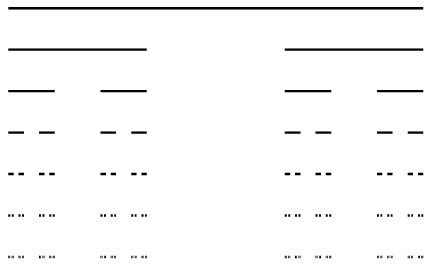
\includegraphics[height=2.5cm, width=5cm]{compact_2.png}$$
\begin{itemize}
    \item Let $E_0 = [0,1]$
    \item Remove the middle third: $E_1 = [0,\frac{1}{2}]\cup [\frac{2}{3},1]$
    \item Repeat: $E_2=\left[0,\frac{1}{9}\right]\cup\left[\frac{2}{9},\frac{3}{9}\right]\cup\left[\frac{6}{9},\frac{7}{9}\right]\cup\left[\frac{8}{9},1\right]$ (still closed, bounded, and compact)\\
    \vdots
    \item Eventually, we get a sequence $E_0 \supset E_1 \supset E_2\supset \ldots$ such that $E_n$ is compact $\forall\;n$.
    \item Hence $\bigcap\limits_{n=1}^\infty E_n \neq \phi$ is compact having infinitely many points.
\end{itemize}
\end{block}

\vspace{1.5\baselineskip}
\begin{block}{\bf Theorem} Let $n$ be a positive integer. If $\{I_k\}$ is a sequence of cube or n-cells such that $I_k\supset I_{k+1}$ (n=1,2,3,...), then $\bigcap\limits_{k=1}^\infty I_k$ is not empty.
\end{block}
$$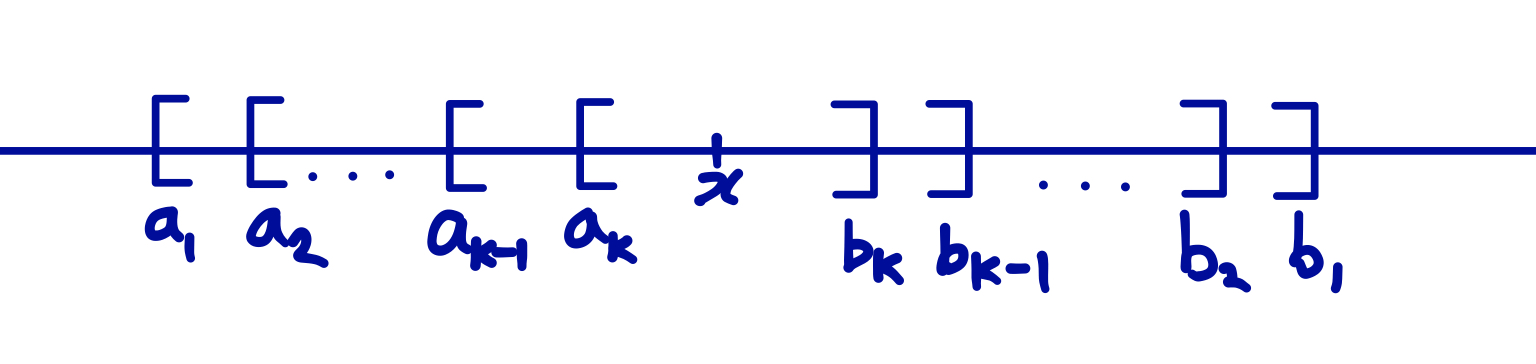
\includegraphics[height=2.5cm, width=15cm]{compact_3.jpg}$$

\vspace{1\baselineskip}
{\sl Proof.}
\begin{itemize}
    \item First, we consider the case $n=1$. So $n-$cells lie in the interval.
    \item So we have $[a_1,b_1]\supset [a_2,b_2]\supset \ldots \;\;$ In particular, $a_k<b_k\le b_1\;\forall \; k$.
    \item So $b_1$ is an upper bound for E. Hence $\exists\; x = sup\; E$
    \item For any $k,m\in\mathbb{N},\; a_k \le a_{k+m} \le b_k$.
    \item So $b_k$ is an upper bound of $E\;\;\forall\;k\in\mathbb{N}$.
    \item Hence $x\le b_k \;\;\forall\;k$ as $x=sup\;E$.
    \item So $a_k \le x \le b_k\;\;\forall\;k\in\mathbb{N}$, so $x\in[a_k,b_k]$.
    \item Hence $x\in \bigcap\limits_{k=1}^\infty [a_k,b_k]$\\
    
    \item Now consider n-cells, $I_1\supset I_2\supset \ldots$ and write $I_k = [a_{k_j},b_{k_j}]\times \ldots\times[a_{k_n},b_{k_n}]$.
    \item Then for each $j=1, \ldots, n$, the intervals $[a_{k_n},b_{k_n}]$ are nested:\\
    $[a_{1j},b_{1j}]\supset [a_{2j},b_{2j}]\supset \ldots \supset [a_{kj},b_{kj}]\supset\ldots$
    \item By first part of the proof, $\exists\;x_j\in\bigcap\limits_{k=1}^\infty [a_{k_j},b_{k_j}]$
    \item Then $x^* = (x_1^*,...,x_n^*) \in \bigcap\limits_{k=1}^\infty ([a_{k_1},b_{k_1}]\times\ldots\times [a_{k_n},b_{k_n}]) = \bigcap\limits_{k=1}^\infty I_k$
\end{itemize}

\vspace{1.5\baselineskip}
\begin{block}{\bf Theorem} n-cells are compact.
 $$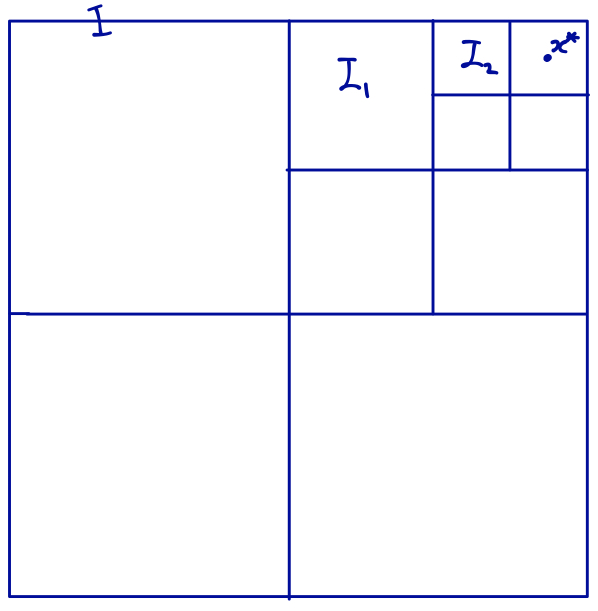
\includegraphics[height=4cm, width=4cm]{compact_4.jpg}$$
\begin{itemize}
    \item Let $I$ be an n-cell, $I = [a_1,b_1]\times \ldots\times [a_n,b_n]$
    \item Define $\delta = \left(\sum\limits_{i=1}^n (b_i-a_i)^2\right)^{1/2}$\quad (max distance between two points.)
    \item Let $\{g_\alpha\}$ be an open cover of $I$.
    \item Suppose by contradiction that there is no finite subcover.
    \item For $j=1,\ldots,n$, let $c_j = \frac{a_j+b_j}{2}$ be the midpoint of $[a_j,b_j]$ can divide to $2^n$ cell.
    \item Divide each interval into $[a_j,c_j]$ and $[c_j,b_j]$ and hence divide $I$ into $2^n$ n-cells.
    \item At least one of these n-cells does not have finite subcover from $\{G_\alpha\}$, call it $I_1$.
    \item Repeating, we get a sequence $I\supset I_1\supset I_2\supset \ldots$ of n-cells such that $I_k$ does not have a finite subcover from collection $\{G_\alpha\}$ 
    \item And if $x,y\in I_k$, then $|x-y|\le \delta2^{-k}$
    \item By the previous theorem, $\exists\; x^* \in \bigcap\limits_{k=1}^\infty I_k$.
    \item As $\{G_\alpha\}$ is an open cover, $\exists\; \alpha_0$ such that $X^*\in G_{\alpha_0}$.
    \item As $G_{\alpha_0}$ is open, $\exists\; r>0$ such that $B_r(x^*)\subset G_\alpha$.
    \item Now as $I_k$ is such that $|x-y|\le 2^{-k}d\;\;\forall\;x,y\in I_k$ taking $k$ sufficiently large so that $2^{-k}\delta < r$, we have $I_k\subset B_r(x_0)\subset G_{x_0}$
    \item As $I_k$ has no finite subcover from $\{G_\alpha\}$.
\end{itemize}
\end{block}

\vspace{1.5\baselineskip}
\begin{block}{\bf Corollary} Every bounded infinite subset $E\subset \mathbb{R}^n$ has a limit point in $\mathbb{R}^n$.
\end{block}

\vspace{1.5\baselineskip}
\begin{block}{\sl Proof.} Since E is bounded, $\exists$ an n-cell $I$ such that $I\supset E$. As $I$ is compact, the infinite subset $E$ has a limit point in $I\subset \mathbb{R}^n$\end{block}

\end{document}